% Provenance (never printed): the households strand of ../economics_series.md (grade 7: income sources, the budget,
% saving, Engel's law; economics only, no advice). Brief: sources/book1/BRIEFS.md, g7-07. Chart data:
% figdata/grade-7/07-households (BLS Consumer Expenditure Surveys 2025, Table 1101; Brenland household survey).
\chapter{Households: Income, Spending and Saving}\label{ch:g7:households}

\begin{openingchart}{Share of yearly spending that goes to four items, for five groups of
households in the United States in 2025: from the fifth with the lowest incomes to the fifth
with the highest, in percent.}{U.S. Bureau of Labor Statistics, Consumer Expenditure Surveys,
2025, Table 1101 (quintiles of \omterm{def:g7:households:income}{income} before taxes)}
\begin{tikzpicture}
\begin{axis}[omrecord, ybar=0.6pt, bar width=6pt, ymin=0, ymax=48,
  symbolic x coords={Lowest, Second, Third, Fourth, Highest}, xtick=data,
  xlabel={Fifth of households, by income}, ylabel={Percent of spending},
  enlarge x limits=0.12, area legend, legend style={at={(0.5,-0.25)}, anchor=north, legend columns=4},
  cycle list={{fill=omDef, draw=none}, {fill=omThm, draw=none}, {fill=omMeth, draw=none},
    {fill=omProp, draw=none}}]
\pgfplotsforeachungrouped \col in {food, housing, health, insurance} {
  \addplot table[x=group, y=\col] {figdata/grade-7/07-households/out/budget_shares.csv};
}
\legend{Food, Housing, Health care, Insurance and pensions}
\end{axis}
\end{tikzpicture}
\end{openingchart}

% figdata: budget_shares (food 13.6 14.5 14.1 13.6 11.5; housing 42.7 ... 30.3; health 10.4 ... 6.2;
% insurance 2 ... 17.7); facts (cex_food_lowest 5156, cex_food_highest 18415)
Every year, a large survey asks \omterm{def:g7:households:household}{households} in the United States what they earn and what they
spend. The chart sorts them into five groups of equal size, from the fifth with the lowest
\omterm{def:g7:households:income}{incomes} to the fifth with the highest, and shows what part of their spending goes to four
items. The poorest fifth spends $42.7\,\%$ of its \omterm{def:g7:households:budget}{budget} on housing, the richest fifth $30.3\,\%$.
Health care takes $10.4\,\%$ at the bottom and $6.2\,\%$ at the top. Food takes $13.6\,\%$ at the
bottom and $11.5\,\%$ at the top, although the richest fifth spends $18\,415$ dollars a year on
food, against $5\,156$ for the poorest. Payments for insurance and into pension systems, most of
them charged on \omterm{def:g7:households:wage}{wages}, take $2\,\%$ at the bottom and $17.7\,\%$ at the top.

Richer and poorer \omterm{def:g7:households:household}{households} do not just spend more or less: they spend in different
proportions. This chapter follows a \omterm{def:g7:households:household}{household}'s \omterm{def:g7:money:money}{money} from where it comes from to where it
goes, and states a regularity found in \omterm{def:g7:households:household}{household} \omterm{def:g7:households:budget}{budgets} everywhere.

\begin{recall}
The \omterm{def:g6:food-and-energy:food-share}{food share} of a \omterm{def:g7:households:household}{household} is its spending on food divided by its \omterm{def:g7:households:income}{income} or its total
spending, and a table must say which (\cref{ch:g6:food-and-energy}); dividing by a reported
\omterm{def:g7:households:income}{income} that is too small can mislead. A \omterm{def:g7:money:price}{price} is an amount of \omterm{def:g7:money:money}{money} given for one unit of a
good (\cref{ch:g7:money}).
\end{recall}

\section{Where income comes from}

\begin{definition}[Household]\label{def:g7:households:household}
A \emph{household}\index{household} is a group of people who live in the same home and share
their \omterm{def:g7:households:income}{income} and their main spending; one person living alone is a household too.
\end{definition}

\begin{definition}[Income]\label{def:g7:households:income}
The \emph{income}\index{income} of a \omterm{def:g7:households:household}{household} is the \omterm{def:g7:money:money}{money} it receives in a period, usually a
year: from work, from a business it owns, from what it owns (interest, dividends, rent), and
from the state. The first three together are its \emph{income before taxes and
transfers}\index{income before taxes and transfers}; what comes from the state is a \omterm{def:g7:households:transfer}{transfer}
(next section).
\end{definition}

\begin{definition}[Wage]\label{def:g7:households:wage}
A \emph{wage}\index{wage} is the pay a worker receives from an employer for work done, by the
hour, the week, the month or the year.
\end{definition}

Most \omterm{def:g7:households:household}{households} live mainly on \omterm{def:g7:households:wage}{wages}. Some own a business, a shop or a farm, and keep what is
left after paying its costs. Some own \omterm{def:g7:households:saving}{savings} that pay interest, shares of firms that pay a part
of their profits, or a flat they rent out. Retired people live on pensions: a pension paid by
the state is a \omterm{def:g7:households:transfer}{transfer}; one paid by a former employer or a pension fund comes from \omterm{def:g7:money:money}{money} put
aside during working years.

\begin{omchart}{Sources of income before taxes, for the same five groups of households in the
United States in 2025, in percent of income. The US survey counts the state's transfers inside
this income: state pensions within retirement pay, benefits within ``other''.}{U.S. Bureau of
Labor Statistics, Consumer Expenditure Surveys, 2025, Table 1101; ``other'' groups public
assistance, unemployment and other benefits, and other \omterm{def:g7:households:income}{income}}
\begin{tikzpicture}
\begin{axis}[omrecord, ybar stacked, bar width=22pt, ymin=0, ymax=100,
  symbolic x coords={Lowest, Second, Third, Fourth, Highest}, xtick=data,
  xlabel={Fifth of households, by income}, ylabel={Percent of income},
  enlarge x limits=0.12, area legend, legend style={at={(0.5,-0.25)}, anchor=north, legend columns=3},
  cycle list={{fill=omDef, draw=white}, {fill=omMeth, draw=white}, {fill=omProp, draw=white},
    {fill=omThm, draw=white}, {fill=black!35, draw=white}}]
\pgfplotsforeachungrouped \col in {wages, business, property, retirement, other} {
  \addplot table[x=group, y=\col] {figdata/grade-7/07-households/out/income_sources.csv};
}
\legend{Wages and salaries, Own business, Interest dividends and rent, Retirement pay,
  Other}
\end{axis}
\end{tikzpicture}
\end{omchart}

% figdata: income_sources (wages 31.2 55.9 75.3 83.4 83.4; retirement 56.4 35.9 17 9 2.8; other 10.4 ... 0.5;
% business 0.5 ... 8.8)
The chart shows that the sources differ along the \omterm{def:g7:households:income}{income} scale. In the poorest fifth, $56.4\,\%$
of \omterm{def:g7:households:income}{income} is retirement pay and $31.2\,\%$ \omterm{def:g7:households:wage}{wages}: many of these \omterm{def:g7:households:household}{households} are retired. In the
richest fifth, \omterm{def:g7:households:wage}{wages} are $83.4\,\%$ and an own business $8.8\,\%$. Many of the poorest \omterm{def:g7:households:household}{households}
are not poor workers but old people who no longer work.

\section{Taxes, transfers and what is left}

\begin{definition}[Transfer]\label{def:g7:households:transfer}
A \emph{transfer}\index{transfer} is \omterm{def:g7:money:money}{money} paid to a \omterm{def:g7:households:household}{household} by the state without any good or
work given in exchange in that period: a state pension, a family allowance, unemployment pay, help
for the poorest.
\end{definition}

\begin{definition}[Disposable income]\label{def:g7:households:disposable-income}
The \emph{disposable income}\index{disposable income} of a \omterm{def:g7:households:household}{household} is its \omterm{def:g7:households:income}{income before taxes
and transfers}, minus the taxes it pays, plus the \omterm{def:g7:households:transfer}{transfers} it receives:
\[
\text{disposable income} = \text{income before taxes and transfers} - \text{taxes} + \text{transfers}.
\]
Each \omterm{def:g7:households:transfer}{transfer} is counted once. A survey that already puts \omterm{def:g7:households:transfer}{transfers} inside its \omterm{def:g7:households:income}{income} before
taxes, as the US survey does, gets disposable \omterm{def:g7:households:income}{income} by subtracting taxes only.
\end{definition}

\omterm{def:g7:households:disposable-income}{Disposable income} is what a \omterm{def:g7:households:household}{household} can actually spend or keep. Its \omterm{def:g7:money:money}{money} then goes two ways:
spent now, or saved for later.

\begin{omfigure}
\begin{tikzpicture}[econ, x=1cm, y=1cm,
  box/.style={draw, rounded corners=2pt, align=center, font=\scriptsize, minimum width=2.6cm,
    minimum height=1cm}]
  \node[box, fill=omDef!15] (g) at (0,0) {income before taxes\\and transfers\\$30\,000$};
  \node[box, fill=omThm!12] (t) at (0,-2.1) {taxes\\$-\,3\,000$};
  \node[box, fill=omMeth!12] (tr) at (3.4,-2.1) {transfers\\$+\,1\,000$};
  \node[box, fill=omDef!25] (d) at (3.4,0) {disposable income\\$28\,000$};
  \node[box, fill=black!8] (c) at (7.4,0.9) {spending\\$26\,000$};
  \node[box, fill=omProp!15] (s) at (7.4,-0.9) {saving\\$2\,000$};
  \draw[-{Stealth}, thick] (g) -- (d);
  \draw[-{Stealth}] (g) -- (t);
  \draw[-{Stealth}] (tr) -- (d);
  \draw[-{Stealth}, thick] (d.east) -- (c.west);
  \draw[-{Stealth}, thick] (d.east) -- (s.west);
\end{tikzpicture}

{\small The \omterm{def:g7:money:money}{money} of an invented Brenland \omterm{def:g7:households:household}{household} over one year, in dalens: \omterm{def:g7:households:income}{income before
taxes and transfers}, minus taxes, plus \omterm{def:g7:households:transfer}{transfers}, gives \omterm{def:g7:households:disposable-income}{disposable income}, which is spent or saved.}
\end{omfigure}

\section{The budget and its shares}

\begin{definition}[Budget]\label{def:g7:households:budget}
The \emph{budget}\index{budget (of a household)} of a \omterm{def:g7:households:household}{household} is the list of what it spends in a
period, item by item, set against its \omterm{def:g7:households:disposable-income}{disposable income}.
\end{definition}

\begin{definition}[Budget share]\label{def:g7:households:budget-share}
The \emph{budget share}\index{budget share} of an item is the \omterm{def:g7:households:household}{household}'s spending on that item
divided by its total spending, often written in percent.
\end{definition}

\begin{example}
The \omterm{def:g7:households:household}{household} of the figure spends $26\,000$ dalens: $6\,500$ on food, $9\,100$ on housing, $3\,900$
on transport and $6\,500$ on everything else. Its \omterm{def:g7:households:budget-share}{budget share} of food is $6\,500 \div 26\,000 =
0.25$, that is $25\,\%$; of housing $9\,100 \div 26\,000 = 0.35$, that is $35\,\%$; of transport
$15\,\%$; of everything else $25\,\%$. The shares add up to $100\,\%$.
\end{example}

\begin{omfigure}
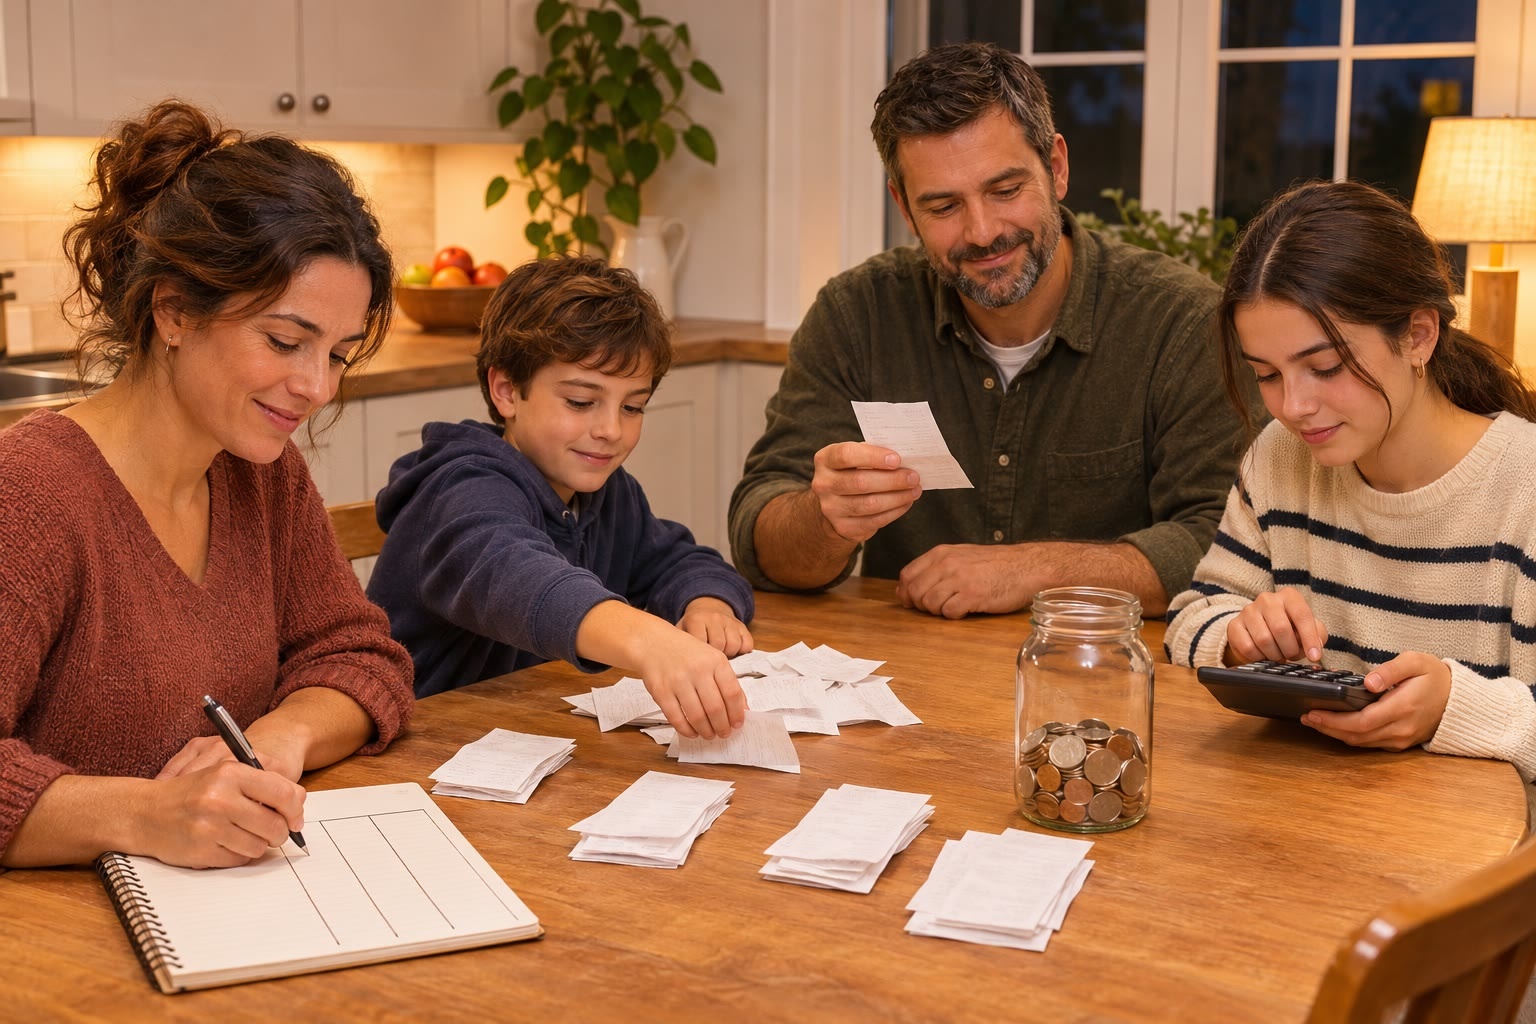
\includegraphics[width=0.52\linewidth]{images/book1/ai/g7-households-kitchen-table.jpg}

{\small Sorting a month's receipts: a \omterm{def:g7:households:household}{household} \omterm{def:g7:households:budget}{budget} is drawn up by putting each spending
under an item and adding up.}
\end{omfigure}

\begin{measure}[A household budget survey]
A \omterm{def:g7:households:budget}{budget} survey chooses \omterm{def:g7:households:household}{households} at random, asks about their \omterm{def:g7:households:income}{incomes}, and asks them to note
every purchase for a week or two, or to recall larger ones over several months. The answers
are weighted so that the sample looks like the whole country. People forget small purchases,
and many report less \omterm{def:g7:households:income}{income} than they have. In the survey of the opening chart, the
poorest fifth reports $18\,125$ dollars of \omterm{def:g7:households:income}{income} before taxes and $37\,935$ dollars of
spending: some of these \omterm{def:g7:households:household}{households} spend \omterm{def:g7:households:saving}{savings}, some receive help from family, and some
report less \omterm{def:g7:households:income}{income} than they receive.
\end{measure}

\section{Saving}

\begin{definition}[Saving]\label{def:g7:households:saving}
The \emph{saving}\index{saving} of a \omterm{def:g7:households:household}{household} in a period is the part of its \omterm{def:g7:households:disposable-income}{disposable income}
that it does not spend in that period:
\[
\text{saving} = \text{disposable income} - \text{spending}.
\]
\end{definition}

\omterm{def:g7:households:saving}{Saving} is spending moved to later. \omterm{def:g7:money:money}{Money} saved this year may pay for a house, studies, a car,
or the years after work. It is often divided by \omterm{def:g7:households:disposable-income}{disposable income}: the \omterm{def:g7:households:household}{household} of the figure
saves $2\,000 \div 28\,000 \approx 0.071$, about $7.1\,\%$ of its \omterm{def:g7:households:disposable-income}{disposable income}. \omterm{def:g7:households:saving}{Saving}
can be negative: a \omterm{def:g7:households:household}{household} that spends more than its \omterm{def:g7:households:disposable-income}{disposable income} draws on its past
\omterm{def:g7:households:saving}{savings} or borrows.

% figdata: engel_quarters (saving_rate 1.8 2.8 5.4 9.9)
In Brenland's \omterm{def:g7:households:household}{household} survey (invented, $2\,000$ \omterm{def:g7:households:household}{households}), the quarter with the lowest
\omterm{def:g7:households:disposable-income}{disposable incomes} saves $1.8\,\%$ of its \omterm{def:g7:households:disposable-income}{disposable income}, the quarter with the highest
$9.9\,\%$. Whether the same holds in a real country is a question for its own survey.

\section{Richer households, different shares}

% ledger: g6:ers-food-share-us-uk, g6:ers-food-share-nigeria, g7:ers-food-dpi-1960, g7:ers-food-dpi-2000,
% g7:ers-food-dpi-2025

\begin{model}{Engel's law}\label{def:g7:households:engels-law}
\assumes \omterm{def:g7:households:household}{Households} first buy the food they need, then spend what is left on other goods; a
person can eat only so much more when richer.
\predicts \emph{Engel's law}\index{Engel's law}: as a \omterm{def:g7:households:household}{household}'s \omterm{def:g7:households:income}{income} rises, its spending on
food in \omterm{def:g7:money:money}{money} rises, but its \omterm{def:g6:food-and-energy:food-share}{food share} falls.
\tested Across countries: food bought to eat at home takes less than $10\,\%$ of \omterm{def:g7:households:household}{household}
spending in the United States and the United Kingdom, and nearly $60\,\%$ in Nigeria. Over time
in one country: as \omterm{def:g7:households:income}{incomes} in the United States rose, food fell from $16.8\,\%$ of \omterm{def:g7:households:disposable-income}{disposable
income} in 1960 to $9.9\,\%$ in 2000. Inside one country in one year the pattern is weak: in the
opening chart food takes $13.6\,\%$ of spending in the lowest fifth and $11.5\,\%$ in the highest,
and $14.5\,\%$ in the second fifth, more than in the first.
\breaks Among very poor \omterm{def:g7:households:household}{households} the \omterm{def:g6:food-and-energy:food-share}{food share} can first rise with \omterm{def:g7:households:income}{income}; in the United
States it has hardly moved since 2000 ($9.7\,\%$ of \omterm{def:g7:households:disposable-income}{disposable income} in 2025); housing does not
follow the same pattern; the share of food eaten away from home rises with \omterm{def:g7:households:income}{income}.
\end{model}

\begin{omchart}{Food share of disposable income against disposable income, Brenland's
$2\,000$ surveyed households (small dots) and the four quarters of households ranked by income
(large squares), invented data.}{Brenland \omterm{def:g7:households:household}{household} survey (the series' invented country)}
\begin{tikzpicture}
\begin{axis}[omrecord, xmin=0, xmax=100, ymin=0, ymax=60, xlabel={Disposable income
  (thousands of dalens a year)}, ylabel={Food share (percent)}, height=0.55\linewidth]
\addplot[only marks, mark=*, mark size=0.5pt, omDef!45] table[x=disp, y=share]
  {figdata/grade-7/07-households/out/engel_points.csv};
\addplot[only marks, mark=square*, mark size=3pt, omThm] table[x=disp, y=share]
  {figdata/grade-7/07-households/out/engel_quarters.csv};
\end{axis}
\end{tikzpicture}
\end{omchart}

% figdata: engel_quarters (disp 14.6 19.9 25.6 39.6; food 3990 4520 4820 5250; share 27.4 22.7 18.8 13.2)
In Brenland, the quarter of \omterm{def:g7:households:household}{households} with the lowest \omterm{def:g7:households:income}{incomes} has a mean \omterm{def:g7:households:disposable-income}{disposable income} of
$14.6$ thousand dalens and spends $27.4\,\%$ of it on food; the quarter with the highest has a
mean of $39.6$ thousand dalens and spends $13.2\,\%$. Yet the richest quarter spends more on food
in \omterm{def:g7:money:money}{money}: $5\,250$ dalens a year on average, against $3\,990$. The dots are scattered: \omterm{def:g7:households:household}{households}
of the same \omterm{def:g7:households:income}{income} differ in size and in tastes. The law is about averages, not about each
\omterm{def:g7:households:household}{household}.

\section{Exercises}

\begin{exercise}[$\star$]\label{exo:g7:households:1}
Use the opening chart. What share of spending goes to housing in the lowest fifth, and in the
highest?
\end{exercise}

\begin{exercise}[$\star$]\label{exo:g7:households:2}
A \omterm{def:g7:households:household}{household} earns $24\,000$ dalens before taxes, pays $2\,500$ dalens of taxes and receives
$1\,800$ dalens of \omterm{def:g7:households:transfer}{transfers}. What is its \omterm{def:g7:households:disposable-income}{disposable income}?
\end{exercise}

\begin{exercise}[$\star$]\label{exo:g7:households:3}
A \omterm{def:g7:households:household}{household} spends $20\,000$ dalens: $5\,000$ on food, $8\,000$ on housing, $3\,000$ on transport and
$4\,000$ on other things. Compute the four \omterm{def:g7:households:budget-share}{budget shares} in percent.
\end{exercise}

\begin{exercise}[$\star$]\label{exo:g7:households:4}
A \omterm{def:g7:households:household}{household} has a \omterm{def:g7:households:disposable-income}{disposable income} of $31\,000$ dalens and spends $28\,500$ dalens. What is its
\omterm{def:g7:households:saving}{saving}?
\end{exercise}

\begin{exercise}[$\star\star$]\label{exo:g7:households:5}
Three Brenland \omterm{def:g7:households:household}{households}: A has a \omterm{def:g7:households:disposable-income}{disposable income} of $16\,000$ dalens and spends $4\,800$ on
food; B, $25\,000$ and $5\,000$; C, $50\,000$ and $6\,000$. Compute each \omterm{def:g6:food-and-energy:food-share}{food share}. Do they
follow Engel's law?
\end{exercise}

\begin{exercise}[$\star\star$]\label{exo:g7:households:6}
Use the Brenland chart and its text. By how many percentage points does the \omterm{def:g6:food-and-energy:food-share}{food share} fall from
the lowest quarter to the highest? By how many dalens does food spending rise?
\end{exercise}

\begin{exercise}[$\star\star$]\label{exo:g7:households:7}
Use the Brenland text. The mean \omterm{def:g7:households:disposable-income}{disposable income} of the third quarter is $25.6$ thousand
dalens and its \omterm{def:g6:food-and-energy:food-share}{food share} $18.8\,\%$. Compared with the first quarter, its \omterm{def:g7:households:income}{income} is about how
many times larger? Is its \omterm{def:g6:food-and-energy:food-share}{food share} more or less than half as large?
\end{exercise}

\begin{exercise}[$\star\star$]\label{exo:g7:households:8}
A \omterm{def:g7:households:household}{household}'s \omterm{def:g7:households:disposable-income}{disposable income} is $2\,400$ dalens a month, and it spends $2\,250$ dalens a month.
What does it save in a year? What part of its \omterm{def:g7:households:disposable-income}{disposable income} does it save, in percent?
\end{exercise}

\begin{exercise}[$\star\star$]\label{exo:g7:households:9}
Describe what a survey would have to show to contradict Engel's law.
\end{exercise}

\begin{exercise}[$\star\star\star$]\label{exo:g7:households:10}
Two \omterm{def:g7:households:household}{households} each have a \omterm{def:g7:households:disposable-income}{disposable income} of $30\,000$ dalens. One has two members, the other
five. The first spends $5\,400$ dalens on food, the second $8\,500$. (a) Compute each \omterm{def:g6:food-and-energy:food-share}{food share}.
(b) Compute food spending per person. (c) Why can comparing \omterm{def:g7:households:household}{households} of different sizes mislead?
\end{exercise}

\begin{exercise}[$\star\star\star$]\label{exo:g7:households:11}
The state gives a \omterm{def:g7:households:transfer}{transfer} of $1\,000$ dalens to two \omterm{def:g7:households:household}{households}. The first, with a \omterm{def:g7:households:disposable-income}{disposable
income} of $15\,000$ dalens, spends $30\,\%$ of any extra dalen on food; the second, with
$60\,000$ dalens, spends $5\,\%$. How much more does each spend on food? Which part of
Engel's law does this fit?
\end{exercise}

\begin{exercise}[$\star\star\star$]\label{exo:g7:households:12}
The opening chart compares different \omterm{def:g7:households:household}{households} in one year. Explain why it cannot tell how the
\omterm{def:g7:households:budget}{budget} of one \omterm{def:g7:households:household}{household} changes when its own \omterm{def:g7:households:income}{income} rises. What data would?
\end{exercise}

\section{Problem: The Brenmoor Household Survey}

\begin{problem}[{Weekend problem --- five households of the survey: income, taxes and transfers;
budget shares and saving; income groups and Engel's law}]
\label{pb:g7:households:1}
% figdata: problem_rows (hh 1 2 4 6 9)
The table gives five \omterm{def:g7:households:household}{households} of Brenland's survey (invented), in dalens a year. \omterm{def:g7:households:income}{Income} is
before taxes and \omterm{def:g7:households:transfer}{transfers}.
\begin{center}
\begin{tabular}{lrrrrrr}
\toprule
\omterm{def:g7:households:household}{Household} & Members & \omterm{def:g7:households:income}{Income} before taxes & Taxes & \omterm{def:g7:households:transfer}{Transfers} & Food & Spending \\
\midrule
A & 4 & 25\,020 & 2\,600 & 2\,400 & 5\,490 & 24\,080 \\
B & 2 & 17\,310 & 1\,060 & 0 & 4\,160 & 16\,250 \\
C & 5 & 19\,400 & 1\,480 & 3\,600 & 6\,890 & 21\,200 \\
D & 3 & 36\,290 & 4\,860 & 1\,200 & 5\,390 & 29\,440 \\
E & 1 & 77\,600 & 18\,760 & 0 & 4\,080 & 53\,060 \\
\bottomrule
\end{tabular}
\end{center}

\medskip
\noindent\textbf{Part I --- Income.}
\begin{enumerate}
  \item Compute the \omterm{def:g7:households:disposable-income}{disposable income} of each \omterm{def:g7:households:household}{household}.
  \item Which \omterm{def:g7:households:household}{household} receives the largest \omterm{def:g7:households:transfer}{transfers}? Which pays the largest taxes?
  \item For \omterm{def:g7:households:household}{household} E, what part of \omterm{def:g7:households:income}{income before taxes and transfers} goes in taxes, in percent?
  \item Rank the five \omterm{def:g7:households:household}{households} by \omterm{def:g7:households:disposable-income}{disposable income}.
\end{enumerate}

\medskip
\noindent\textbf{Part II --- Spending and saving.}
\begin{enumerate}[resume]
  \item Compute the \omterm{def:g7:households:saving}{saving} of each \omterm{def:g7:households:household}{household}.
  \item Compute the \omterm{def:g6:food-and-energy:food-share}{food share} of \omterm{def:g7:households:disposable-income}{disposable income} of each \omterm{def:g7:households:household}{household}, rounded to one decimal.
  \item Which \omterm{def:g7:households:household}{household} saves nothing?
  \item Compute the \omterm{def:g7:households:saving}{saving} of D and of E as a part of their \omterm{def:g7:households:disposable-income}{disposable income}, in percent.
\end{enumerate}

\medskip
\noindent\textbf{Part III --- Income groups.} The whole survey ($2\,000$ \omterm{def:g7:households:household}{households}) is split into
four quarters by \omterm{def:g7:households:disposable-income}{disposable income}. The quarter with the lowest \omterm{def:g7:households:income}{incomes} has a mean \omterm{def:g7:households:disposable-income}{disposable
income} of $14.6$ thousand dalens, mean food spending of $3\,990$ dalens and a \omterm{def:g6:food-and-energy:food-share}{food share} of
$27.4\,\%$; the quarter with the highest, $39.6$ thousand, $5\,250$ and $13.2\,\%$.
\begin{enumerate}[resume]
  \item Do the five \omterm{def:g7:households:household}{households} of the table follow Engel's law? Name the \omterm{def:g7:households:household}{household} that departs
        most from it, and give one reason from the table.
  \item Compute food spending per member for \omterm{def:g7:households:household}{households} C and E.
  \item How many times larger is the mean \omterm{def:g7:households:disposable-income}{disposable income} of the top quarter than that of the
        bottom quarter? And its food spending?
  \item Using the quarters, state Engel's law with the numbers: what happens to food spending, and
        to the \omterm{def:g6:food-and-energy:food-share}{food share}, from the bottom quarter to the top.
\end{enumerate}
\end{problem}
